\section{多次反射处理方法的前景}
\label{sec:5.6}

要改善压制多次波的能力,我们就得力争比较好地描述其特征,麻烦的是实际模型总是
有许多的组成因素。在丰富的文献中几乎没多少理论已经对日常的生产实践有很大影响,我
把那些不成功的理论分成两类:
\begin{enumerate}
\item 试图以统计方法解决每个问题,把空间关系过分简化了的那些理论;
\item 试图以数学物理方法解决每个问题,把资料的不完全性质和干扰性质过分简化了
的那些理论。
\end{enumerate}

对于进入地球物理领域的原子核物理学家、天体衡理学家和数学家来说,多次反射是一
个很合适的题目。那些愿意接受挑战、力图坚持理论联系生产实践的人们学会谦虚谨慎一些
就能得到报偿。我愿现在告诫你们,在这节中我始终还未曾把它们拉扯在一起!

本节将提出两种处理办法,这二者均注重几何方法和统计方法,两种办法都是新方法而
且没经过多少检验,不论它们如何能起良好作用,我想你们会发现它们对解决这个任务总是
有所启发的。

第一种方法称作共中心点倾斜叠加(CMP slant stack),这是其中简单的一种方法,
它将资料变换成这样一种彤式:其中所有炮检距上的记录道均是模仿简单的一维零炮检距模
型,关于该种模型的文献在数学物理和统计学中是很广泛的。

第二种方法是以置换阻抗(replacement inpedance)概念为基础,设计它的意图是为了
适应近地面的快速横向变化。用假想的海上环境条件最容易解释这种方法的意义,其中产生
的唯一困难就是海底反射率之横向变化。方法的基本思想是将定向的炮点与定向的检波点向
下延拓至不多不少正好在海底之下,然后经由一卜具有零值海底反射系数的置换介质向上延
拓;这种处理过程不会消除所有的多次反射,但是它应能消除最令人恼火的一些多次波。

\subsection{以倾斜叠加方法变换至一维情形}
\label{sec:5.6.1}

关于多次反射的一维模型,现在有丰富的文献,一些著者发展了波动传播理论的许多分
支方面的工作,另一些著者则从简化传播模型开始着手,发展了信息论的许多分支方面的工
作。这些一维理论总是被认为只能应用于零炮检距情形,其实,我们将会看到,以倾斜叠加
作为工具是可以使所有其他炮检距情形都能进入一维问题领域的。

有一种途径可以像垂直入射情形下那样计算出多次波的时间关系和振輻关系,这就是不
再把地震记录考虑为恒定炮检距情形下的时间函数而开始考虑恒定Snell参量时的情形。在
分层地层内,完整的射线路程是把各层内的路程相加而构成的。在垂直入射时$p=0$,显然可
知,当射线位于第i层内的时候,它在该层内的旅行时间L是独立于总旅程中其他微屈多次反
射路程的。对于任何其它固定参量办旅行时间的这种独立性同样也成立。但是,如图\ref{fig:mltp/multangle}
所示,在射线的总偏移距$\sum f_j$是固定而不是p值固定的情形下,这稗性质就不成立了。与此
情开彡类似,在p值固定情形下,射线在第纟层时传播经过的水平距离$f_i$是独立于总旅程中其它
微屈路程的,因此,就任何第i层而言,时间$t_i$+常数$\times f_i$应独立于总路程中的其它微屈多
次反射的路程。所以,$t_i'=t_i-of_i$是表现第i层的一种特性而且它与可能位于总路程中的任
何其他地层均无关。已知射线通过各地层后,你就能将各层相应的$t_i$和$f_i$加起来,就象你在
垂直入射情形下要作的那样。

\begin{figure}[H]
\centering
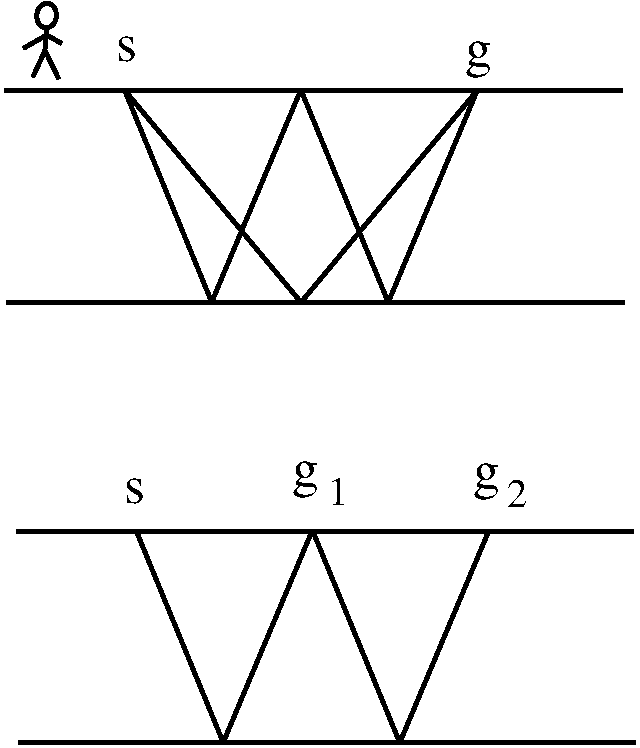
\includegraphics[width=0.65\textwidth]{mltp/multangle}
\caption[multangle]{到达恒定炮检距的射线具有各种不同角度,因而也就是具有各种不同Snell参
量(左图)。具有恒定Snell参量的射线到达时,可以有各种不同的炮检距(右
图),Snell参量p值恒定时,所有各个路程均有相同旅行时间
}
\label{fig:mltp/multangle}
\end{figure}

为了解野外资料是如何同倾斜叠加联系起来的,需从在共中心点道集上搜索那些在双曲
线波至达到某个特定鋇率值$p=dt/df$之处的所有能量开始说起,地面覌测资料上所见的这些
能量片断,每个都可告诉我们具有该Snell参量p的射线是在何处和何时到达地靣的,典型的
几何关系和合成数据如图\ref{fig:mltp/intervalvel1}和图\ref{fig:mltp/intvel2}所示。



\begin{figure}[H]
\centering
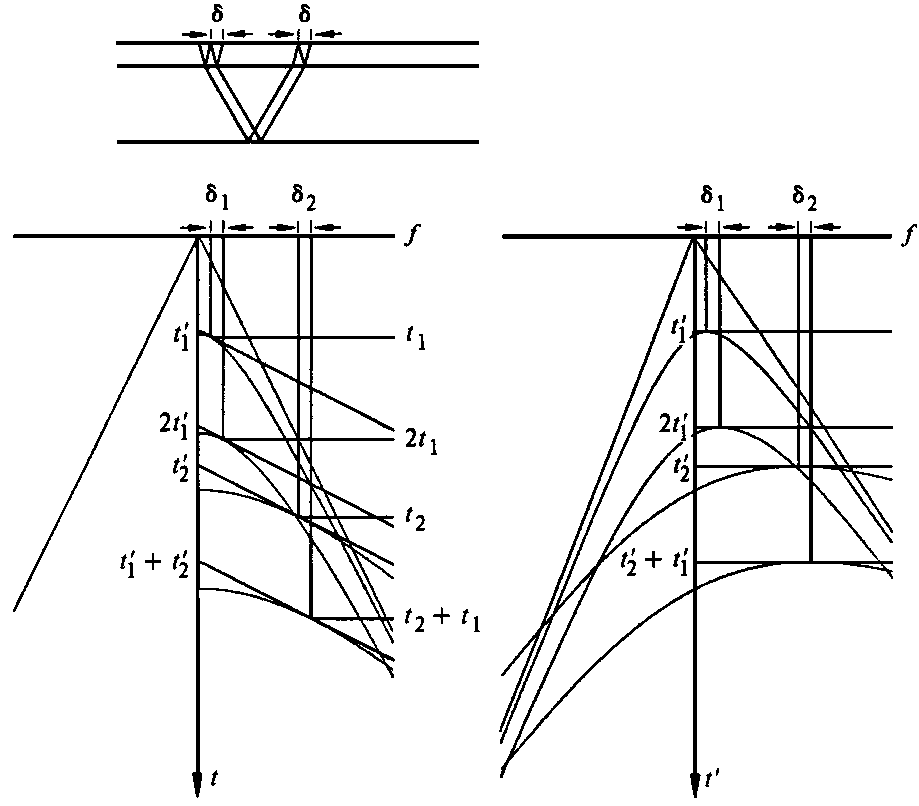
\includegraphics[width=0.65\textwidth]{mltp/intervalve1}
\caption[intervalve1]{表示同相轴$(t_1,2t_1,t_2,t_2+t_1)$的二层模型。
顶部图是射线路程,左图是通常的数据道集,右图是该道集经过线性时差校正$t'=t-pf$
之后重新显示的结果。各图系按比例为$(1,2,3)$的参量$(v_1,v_2,1/p)$计算出来。注意与斜率为p之直线相切处的
同相轴片断,我们看得出到达时间有垂直入射时的关系---就是说,混响周期是固定的。而且对微屈多次
波和对简单多次波都一样。之所以必然如此,是因为顶部的图中之射线路程可以精确地应用于那些在
出之处的同相轴片断;此外,由于$\delta_1=\delta_2$,时间$(t_1',2t_1',t_2',t_2'+t_1')$也是同熟悉的垂直入
射模式一样(据Gonzalez)
}
\label{fig:mltp/intervalve1}
\end{figure}

\begin{figure}[H]
\centering
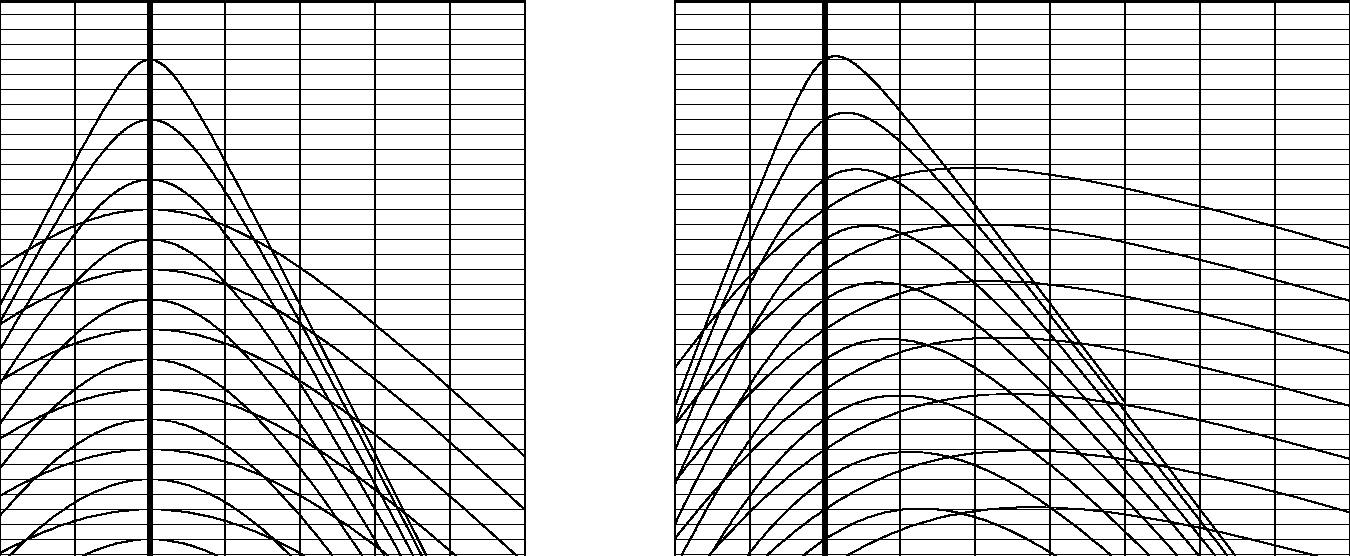
\includegraphics[width=0.65\textwidth]{mltp/intvel2}
\caption[intvel2]{
除表示出有更多多次反射之外,此图与图\ref{fig:mltp/intervalvel1}
是相同的
}
\label{fig:mltp/intvel2}
\end{figure}

$t_i$与$t_i'$二者的行为性质都像法线入射多次反射的时间。尽管任何能量片断之横向位置令
人遗憾地是与速度模型$v(z)$有关,可是进行倾斜叠加却无关于横向位置。原则上,可以用
许多离散的p值完成倾斜叠加,使$(f,t)$空间映射为$(p,t)$空间。利用$(p,t)$空间妙就妙
在多次波压制问题可以分解成许多单独的一维问题,每一个力值各相应于一个问题;不仅如
此,而且求解这些问题不需要已知地层速度,反倒轮到由你从已公布的许多方法中去挑选你
爱用的方法了。在压制多次波之后,你就作逆倾斜叠加,一旦变回至$(f,t)$空间,你就能
佶计速度并利用你拿手的叠加方法进一步压制多次波。

图\ref{fig:mltp/intvel2}是一种“工作手册”式的练习。把右图中所有同相轴的顶部挑出来,然后用虚
线把它们联起来,你就能够证实海底微屈多次波具有像简单樺底多次波一样的层速度。沉积
地层的层速度可由一次波测定出,将第n简单多次波与第n微屈多次波联起来也可以测定出沉
积地层的速度。

用反褶积方法消除交混回晌的办法坷利用倾斜叠加变换至一维问题情形来代替,例如,
可参阅Treitd等人的论文(1982
)。这是介于试验研究工作与工业生产实践二者之间的一
项矬理方法,有待进一步完善。它的强有力之处在于它既正确地掌握了固有的反射系数之角
度依赖关系,又正确地掌握了由炮点与检波点之几何分布形式所形成的角度依赖关系。它的
弱点之一是它假设产生混响的地层内具有横向均勻性,海水层倒是极均勻的,但是海底沉积
物却可能相当不均匀。

\subsection{近地表不均匀性}
\label{sec:5.6.2}

土壤层具有奇怪的声学性质,地震波在其中的传播速度一般小于或等于水中的声速1500
米/秒;土壤层的速度比水中声速低五倍、即像空气中的声速一样慢(
300米/秒),也并非
少见的事。实际工作时,地震震源均埋置于风化带之下。除了在沼泽地区外,接收器大多总
是必须置于风化带之上,在沼泽区的野外工作非常困难,以致你要比平常少用许多检波器。

非常困难的根源在于土壤层是显著横向不均匀的。两个相距不过10米的检波器得出很不
相同的地震记录,并不稀罕。尤其是,井口时间(由炮井底部至井顶附近地面的地震波旅行
时间)可以很容易显示出相当于整个波长的时间异常,尽管实际是平坦水平的地面,对风化
带内有如此明显而不可预测的旅行时间异常如何理解呢?这得用河流蛇曲、超浅层气藏、碳
酸盐岩溶洞、冰碛物等等的影响去解释,所有这些不规则性影响在深部虽也能发现,但是只
要含水饱和度和地下压力并未减小阻抗的非均匀性,那么在近地表处的那些不规则性影响就
更严重。关于这个问题尚可参阅\ref{sec:3.7}节的论述。

浅海情形要好一点,横向变化仍存在有充分机会---那里不但有埋藏的古河道而且还有
埋藏的海底水道,但是浅海情形的主要问题变成了海水层的鸣震问题,观测资料的功率谱将
受这种鸣震所控制。

与此情形类似,对陆地资料而言,功率谱总是逐个记录站而迅速变化的,谱的这些变化可
解释为多次反射之变化,而多次反射之变化则是由有效深度或风化带特征之变化所引起的。

\subsection{模拟时应注意之点}
\label{sec:5.6.3}



向下延拓方程包含四种主要因素:检波点处介质之慢度$1/v(g)$;炮点处介质之慢度
$1/v(s)$;炮检距空间内之时差$k_h/\omega$;中心点空间内之倾角$k_y/\omega$。这四种因素均具有相同
物理量纲,因而按照假设存在于各因素之间的数值不等式关系可以将模拟处理过程加以分
类。一维工作忽略四种因素中的三种,即倾角、时差和差值$v(g)^{-1}-v(s)^{-1}$。
共中心点叠
加包括时差$k_h/\omega$,关于是否包括倾角或横向速度变化,我们现在可以有选择的自由;横向速度
变化往往是在存在有微屈多次波的地表面附近十分显著;记住来自深部地下界面的典型情形
是射线以陡角度在低速地面出射这个简单概念,当在近地面处应兩延拓方程时,由于应有
$1/v>>k_y/\omega$,略去倾角是特别正确的。既然我们的野外工作极难控制超岀射线平面之外的倾
角,最好是找到这种可以略去倾角的借口
。另一方面,炮检距空间的时差大概总是在射线平
而之内要比在射线平面之外大很多。

对多次反射进行模拟或处理时,另一种重要因素是上行波与下行波的耦合作用。这种耦
合作用引进了在炮点下方的反射率$c(s)$和检波点下方的反射率$c(g)$。以后我们还会讨论的
一个重要可能性就是:纵使所有角度均能忽略,$c(s)$还是可能不同于$c(g)$。

\subsection{多次反射相减消去法}
\label{sec:5.6.4}

进行叠加可看作是加法过程,进行模拟则导至减法处理,该减法过程是对叠加的补充而
不是替换物:在相减之后,你就可叠加。

首先我们试图模拟该多次反射,然后我们试图从数据中把它减掉。一般而言,用减法消
除多次波比用加法消除多次波有更多危险。为成功地运用减法,不但要求时间误差小于四分
之一波长而且要求有正确的振幅。

为考虑说明模拟结果与现实之间的偏差,可引入以统计方法确定的经验常数。在统计学
中,这种方法以回归方法而知名。例如,已知数据点集合应拟合于某一直线时,我们即可对
残差利甩最小二乘法确定该直线的最佳参量。这样,移去该直线,就可以开始仔细研究这些
数据点了。这非常像我们打算进行的多次反射消除,如有可调参量自然可以更有助于考虑在
计算精确多次波振幅时可望遇到的困难。未知的时间误差非常难以模拟。因为存在有数学上
的非线性性质,有种稍微不同但更易于控制的办法,就是将褶积滤波中的系数取为可调参
量,这样一种滤波可以代表任何比例因子和时移。采用时变滤波来计算时变模拟误差,是引
人感兴趣的办法。采用这种办法时逃避不了的一个困难是:一项滤波因子可能代表一大堆东
西而不仅限于标定和振幅。你采用的参量越多,模型就将越能拟合于数据,不论该模型是否
真正地与数据有关。

将多次反射减去时所发生的困难实际上仅仅是这样:模拟多次波时---比方说,模拟其
几何分布或速度时---如果有不合适之处,这时你需要在回归方法中利用许多可调参量进行
适当的补偿,而采用很多可调参量,就不但减去了多次波而且还可能减掉了一次波,这真是
泼洗澡水连孩子也一块泼出去了!

\subsection{倾斜反褶积与反演}
\label{sec:5.6.5}

因为实际工作采用宽炮检距,事情已日益明显,地震学家必须逐个研究多次反射并注意
海底的差异。Taner (1980)曾介绍过一种可以如此作的直接而又吸引人的方法,那就是他
的径向记录道法(radial-trace method),径向记录道是沿恒定值$r=h/t$的某条直线斜穿
过共炮点道集的一条直线。我们不对恒定炮检距上的记录道进行反褶积,而对径向记录道采
用反褶积。反褶积可推广至向下延拓过程,径向记录道的向下延拓能用时移来近似。可惜,
当直线上的数据是由海底多次波和微屈多次波组成时会出现问题,因为这些多次波要求有不
同的轨线,以Snell波为工具是可以解决这个问题的,至少在原则上可以如此。Estevez
(1977)在其学位论文中从理论上证明了Snell波如何也能用于解决像绕射与横向速度变化
(如果已知)这类困难。Estevez的论文中有个阐明海底深度相异对不同多次反射有密切影响
的例子,如图\ref{fig:mltp/estevez}所示。

\begin{figure}[H]
\centering
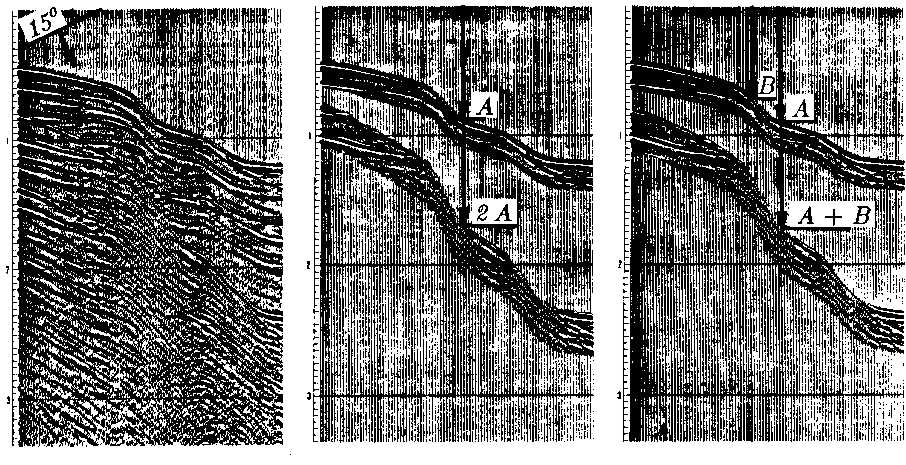
\includegraphics[width=0.65\textwidth]{mltp/estevez}
\caption[estevez]{
多次波之时间与所有时间之和有关(据Estevez )
}
\label{fig:mltp/estevez}
\end{figure}

大多数反演赴理所面临的问题都是由资料缺乏完整性引起的,资料可能是在时间和空间
方面或在它的谱方面不完整。对任何递归方法均须加以认真分析,以保证在浅层深度上所造
成的误差不至于在继续往下算时会不受控制地发生混合。一切资料在谱方面都是不完整的,
还有,利用一切资料时都有个关于爆炸波形的不确定性问题。在值受到微屈多次波的不利
影响时,第一个海底反射通常出现在过于靠近勘探船之处,严格来说是记录不到的。为解决
这个问题,Taner建立了一种特殊辅助记录系统。

Snell波方法有个好处,进行倾斜叠加就能由原始野外资料形成某种信噪比増强,但是
它也有个不利之处,向下延拓必须一直进行到所有深度。以后所要讨论的一些方法均属叠前
方法,不过它们并不要求向下延拓到低于海底。

\subsection{分裝法Backus滤波}
\label{sec:5.6.6}

为了处理地面多次反射,我们准备提出一种普遍性的策略、即阻抗置换方法.这种策略
将需要以回归理论和波场延拓理论作为重炮武器,为了不至于迷失目标,我们将用取自理想
化几何关系的一个例子来开始着手讨论。Larry
Morley曾以实例说明实际情况与这种理想
化精形相距并不太远,其博士学位论文(1982
)阐述了应用这种方法的一项成功试验并详细描述了阻抗置换的策略。

试想像海底是平坦的,取炮点附近的海底反射系数为$c_s$,在检波点附近则取为$c_g$,检波
点附近的混响模式为
\begin{equation}
\frac{1}{1+c_gZ}=1-c_gZ+c_g^2Z^2-c_g^3Z^3+c_g^4Z^4+......
\label{eq:ex5.6.1}
\end{equation}
式中,Z为传播至海水层底部情形下的双程延迟算子(见\ref{sec:4.
6}节或《地球物理数据处理基础》
一书关于Z变换背景的讨论)。在炮点附近有类似的混响序列:
\begin{equation}
\frac{1}{1+c_sZ}=1-c_sZ+c_s^2Z^2-c_s^3Z^3+c_s^4Z^4+......
\label{eq:ex5.6.2}
\end{equation}
忽略G与q之间的差别,则导至Backus混响序列,它是式\ref{eq:ex5.6.1}与式\ref{eq:ex5.6.2}的乘积。

\begin{equation}
\frac{1}{1+cZ}\frac{1}{1+cZ}=
1-2cZ+3c^2Z^2-4c^3Z^3+5c^4Z^4+......
\label{eq:ex5.6.3}
\end{equation}

式\ref{eq:ex5.6.3}左端的分母就是Backus滤波算子,采用这个滤波算子应可消除混响序列。
Morley将明显包含炮点与检波点之差异所形成的该种滤波算子称为分裂法Backus滤波。深
度以及反射系数均可能横向变动(倾角影晌是二阶量),于是分裂法Backus算子可取为:
\begin{equation}
(1+c_se^{i\omega\tau(s)})(1+c_ge^{i\omega\tau(g)})
\label{eq:ex5.6.4}
\end{equation}
求式\ref{eq:ex5.6.4}的倒数,将它展开成类似于式\ref{eq:ex5.6.3}的表达式,你就会发现第n项分裂成n个
项了,这正是意味着炮点附近海底反射的路程可以具有不同于检波点附近海底反射路程的旅
行时间。


下面的图\ref{fig:mltp/splitpeg}取自Morley的学位论文,它表明分岔的微屈多次波是一种可观察到的现
象。他对该图有下列解释:

该图系偏移距略小于电缆长度二分之一情形下取自同一测线的共炮检距剖面(COS
)(偏移距为45个炮点)。在左侧2.5秒时开始一直延续至右侧3秒时的一阶微屈多次波在近
记录道剖面上是“蜕化”的(未分岔),而在这个COS剖面上则由于受海底地形影响却是分
岔的,最大分岔出现在炮点180至200附近,约为200毫秒。正如人们所预料,这最大分岔出
现在海底具有最大倾角之处,即炮点位置与检波点位置上饰海底深度之差为最大之处。

\begin{figure}[H]
\centering
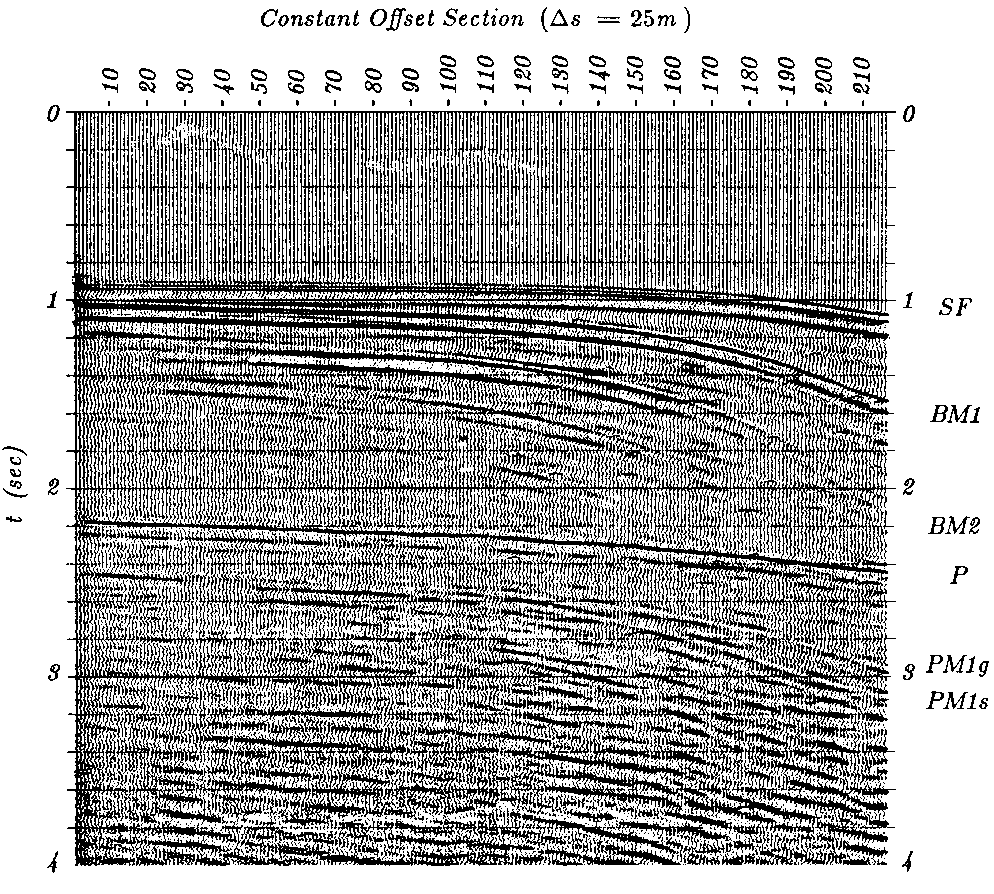
\includegraphics[width=0.65\textwidth]{mltp/splitpeg}
\caption[splitpeg]{
共炮检距剖面(COS),所在测线与\ref{sec:5.5}节中之图\ref{fig:mltp/nearoffset}的测线相同,偏移距
约为45个炮点距离.注意,一阶微屈多次波现在分岔成为两个明显可区别的波
至$PM_{1s}$和$PM_{1g}$ (据Morley )
}
\label{fig:mltp/splitpeg}
\end{figure}

目前大多数处理方法均完全忽略了Backus滤波而对每个地震记录道采用独立的反褶积
滤波求解办法,这种作法引入了大量自由参量,与此相比之下,分裂法Backus滤波处理办法
在保存一次波方面应能起比较好的作甩。

在实际应用时,我们预料任何以分裂法Backus滤波概念为基础的方法将需要包括时差校
正影响。很幸运,速度差异会减小微屈多次波的出射角。当然了,剩余时差问题会使海水层
底部多次波成为一种非常麻烦的事,在那种场合下,大概是应当在正常时差校正之后才能应
用该种处理。以下让我们考察一下对分裂法Backus算子作估计的问题。

% \subsection{浅水多次波聚焦现象的例子}
% \label{sec:5.5.7}

% 爆炸反射面概念不能应用于多次反射,所以不存在什么可以在近记录道剖面上预测多次
% 波之聚焦冇为表现的简单波动理论手段工具。幸好垂直平面波叠加剖面中之多次波是可分析
% 的,它们能够给我们提供关于其他迪震剖面上多次反射之聚焦行为表现的某种概念。垂直下
% 行平面波可用无时差校正的共检波点叠加来模拟,这种共检波点叠加并不与熟悉的共深度点
% 叠加(CDP)相同,但却可用第一章与第二章中所述技巧对它进行分析。

% 试考虑一下经历过若干次由地面发生反弹的多次反射。一开始传播的时候,它是一个下行
% 平面波,如此保持不变,直至它由海底发生第一次反射。海底的反射使该平面波受到了海底
% 地形的影响,利用透镜项方程能在计算机内模拟地形对平面波的这种影响,这时由海底各点
% 形成绕射,向上传播至地面,然后又反射向下至海底,于是再应用透镜项方程在计算机内又
% 一次模拟出因海底地形影响而出现的时移。如此交错采用绕射和地形透镜时移
% (topographic lens shift)的过程能随你所愿地重复进行。图5.
% 5-10所示就是这样一种模拟结果,图\ref{fig:mltp/simulated}中的
% 高阶多次反射之突出特征是能量集中在局部化区域内,很容易看出海底凸出部分的反射如何
% 能够克服地震波能量扩散开来的趋势,时间坐标轴较深部位上出现的这些能量高度集中区完
% 全不像一次波,对一次波来说,局部化扰动应有扩散开来成为宽阔双曲线同相轴的趋向。如
% 若对图\ref{fig:mltp/simulated}中所见那些能量高度集中点像对一次波那样作偏移,必然是形成半圆弧形,这类
% 半圆弧形丝毫也不像是什么地质模型,而且即使采用生产应用上最佳的偏移程序处理,也完
% 全不会使结果有什么改变。

% 从图\ref{fig:mltp/simulated}的合成多次及射得到的最重要经验就是:多次波并不需要与一次波相似。偏
% 移叠加剖面上出现的半圆弧形同相轴可能是剩余多次反射,可惜,还没什么简单理论可以说
% 明垂直平面波叠加剖面上的聚焦多次波是否应
% 当类似于零炮检距剖面或CDP叠加剖面上的那
% 些多次波。幸亏还存在有可以提供答案的一些资料,图\ref{fig:mltp/multfoc2}是一个零炮检距剖面,它证实 在反射法勘探资料上如果不是以定量方式至
% 少也是以定性方式确实可以发现此类聚焦现象。

% 图\ref{fig:mltp/multfoc2}展示的海上勘探资料清楚地显示
% 出图\ref{fig:mltp/simulated}合成记录计算中的聚焦现象,这使
% 我们想到,为了得到清晰的地下界面图像,应
% 当以定量方式利用我们对此问题的理解。但是
% 有若干原因使我们作不到这点,第一,Riley
% 的理论只适用于垂直平面波叠加剖面,这些剖
% 面在定量上就不同于共中心点叠加剖面;第
% 二,地震剖面上海底的实在深度是未知数,它
% 必须根据数据资料本身以某种什么方法来确定;第三,图\ref{fig:mltp/simulated}中的海水深度太浅,以致各个单独反射无法加以区别。

% \begin{figure}[H]
% \centering
% 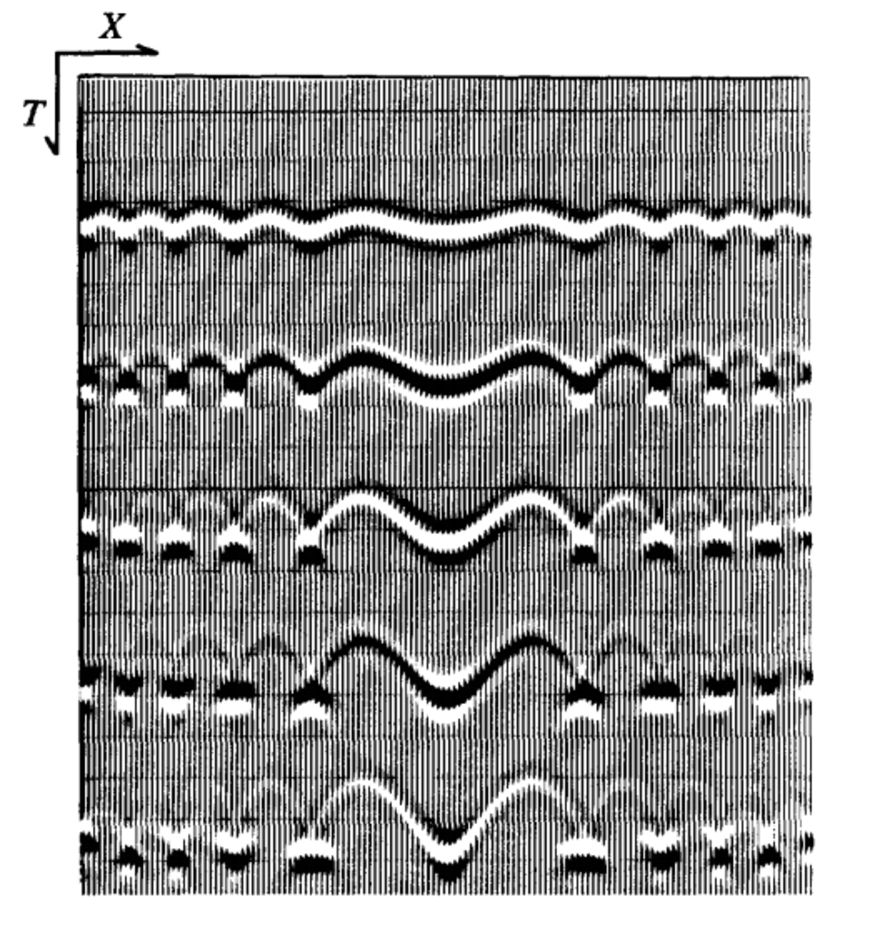
\includegraphics[width=0.65\textwidth]{mltp/simulated}
% \caption[simulated]{
% Chukchi海地区近记录道剖面中的聚焦作用对多次反射影响的例子,
% 这些影响为叠加所掩盖(据美国Geological Survey)。A. 现
% 存的构造;B. 以前的构造已不均匀侵蚀掉,留下海底的局部性
% 凸起或凹下;C. 高阶多次反射在海底凹下之处聚焦;D. 暴露在
% 多次波微弱之处(即海底凸出引起多次波迅速扩散之处)的时窗
% 内之现存构造倾角
% }
% \label{fig:mltp/simulated}
% \end{figure}

% \begin{figure}[H]
% \centering
% 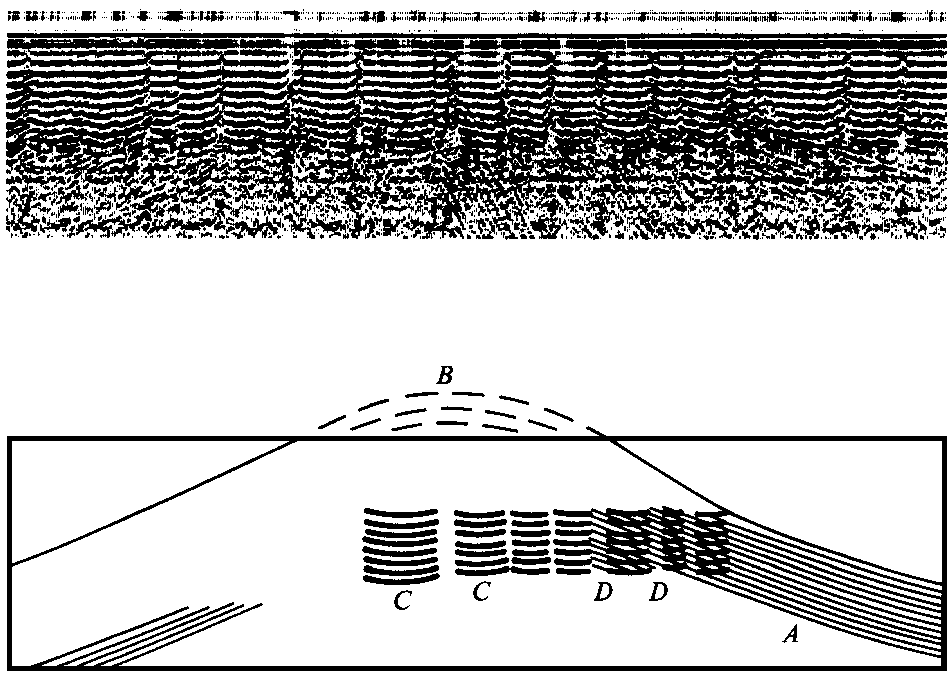
\includegraphics[width=0.65\textwidth]{mltp/multfoc2}
% \caption[multfoc2]{
% 绕射多次反射例子:(a)一维合成记录。(b)二维合成记录,垂直平面波震源。
% (c)27次覆盖CDP剖面。(d)近记录道剖面(据Riley)
% }
% \label{fig:mltp/multfoc2}
% \end{figure}

% \subsection{反褶积为何在深水情形下失败}
% \label{sec:5.5.8}

% 在深水情形下,反褶积处理一般是无效的,这已是众所周知的了。所以如此,有一个可
% 能原因,即深水条件并不是多次反射问题等价于爆炸波形问题的数学极限条件;不过,事情
% 还不完全仅限于此。

% 理论预言多次波在普通环境条件之下应有极性交错变化。图\ref{fig:mltp/multiple}和图\ref{fig:mltp/gsidecon}的例子证实
% 了这点,你也许已注意到,这种极性交错变化可能很难在CDP叠加资料中观察出来,但是在实
% 际工作中,如果条件顺利,还是容易观察到的。尽管图\ref{fig:mltp/nearoffset}的图幅较小,你在图中还是能
% 看出它的。在浅水中,各个脉冲到达时间太靠近,没法把它们区别开来;或者炮检距所张角
% 度成了掠射角,而理论预言在超过临界角时会有不同于$\pi$的相移,因此你在那种情形下见不
% 着简单的极性交错现象是理所应当的。在深水中,脉冲均彼此可区别,在最近的炮检距上应
% 可观察到极性交错,但是要在共中心点叠加剖面上寻找交错的极性,那你就会碰到麻烦,这
% 也就是用反褶积方法从共中心点叠加剖面中消除深水多次波为什么会趋于失败的原因。

% 回想一下各多次波在零炮检距上的时间关系。混响周期按说是常数,但因为有正常时
% 差,在任何其他炮检距上情形却并非如此。正常时差校正能成功地在恒定速度地层情形下恢
% 复零炮检距上的时间关系,但是在速度随深度而增大时,多次波所具有的均方根速会将比一
% 次波均方根速度低,因此,成问题的是采用什么速度以及在典型的陆地与海上勘探情况下剩
% 余时移是否大于半波长。回答这个问题不需要求解什么方程,只需全面观察常规共中心点叠
% 加能压制多次波就是因为多次波具有比一次波为低的速度,这种观察说明正常时差校正照例
% 是使多次波具有超出其自然零炮检距关系半个波长左右的时移。

% 我们所期望之零炮检距上的振幅关系出现混乱,会使事情变糟。反射系数是反射角度之
% 函数,可是从某个特定炮检距上的地震记录开始,各个多次反射就会已经是以不同的角度反
% 射的了。

% 垂直入射的时间关系是近似显示在共深度点叠加剖面上的,实际应用时的困难在于,共
% 深度点叠加模仿垂直入射情况还没完美到足以使人能够满意地从一次波预测出多次波。

% 在叠加以前,对海上资料可以采用海水速度完成时差校正,但这时任何微屈多次波就会
% 不适用于法线入射的时间关系了,既然微屈多次波是多次反射问题中最难处理的部分,也许
% 是应该以微屈多次波的速度来完成时差校正才好,不管你如何考虑这问题,反正所有深水多
% 次反射的时间关系严格说都不可能用时差校正的办法来调整。

% \subsection{习 题}
% \label{sec:5.5.9}

% \begin{enumerate}
% \item 在某种陆地勘探资料上已经注意到有这种现象,即深水多次反射到达时间比理论
% 所预言的时间要稍微早一点,试问这种现象应如何解释?
% \end{enumerate}